\documentclass[convert = false, tikz]{standalone}
\usepackage[utf8]{inputenc}
\usepackage{tikz}
\usetikzlibrary{automata, positioning, arrows}
 
\usepackage{../../../../style_automata}

% arara: pdflatex
% arara: latexmk: { clean: partial }
\begin{document}
    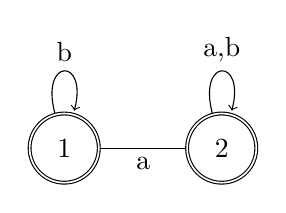
\begin{tikzpicture}
        \tikzset{
        node distance=2cm, % specifies the minimum distance between two nodes.
        }
        \node[state, accepting] (t1) {$1$};
        \node[state, accepting, right of=t1] (t2) {$2$};
        \draw (t1) edge[loop above] node{b} (t1)
        (t2) edge[loop above] node{a,b} (t2)
        (t1) edge[below] node{a} (t2);
    \end{tikzpicture}
\end{document}
